\chapter{Caracterización del  Electroimán} \chapterlabel{Informe/3-CaracterizaciónElectroimán} \label{cap:CaracterizaciónElectroimán}

\section{Caracterización del Electroimán}

\noindent El actuador de este sistema de control es un electroimán. Se eligió construirlo utilizando un núcleo de acero al silicio con un bobinado en su interior. 
%mejorar esto

\noindent Se puede modelar el problema como un objeto de masa puntual que es sometido a dos fuerzas opuestas en el eje “Y” de la figura \ref{fig:img_modelado-fisico}: la de su propio peso hacia abajo, y una fuerza realizada por el electroimán en sentido contrario.

%capaz poner otra imagen
\begin{figure}[H]
	\centering
	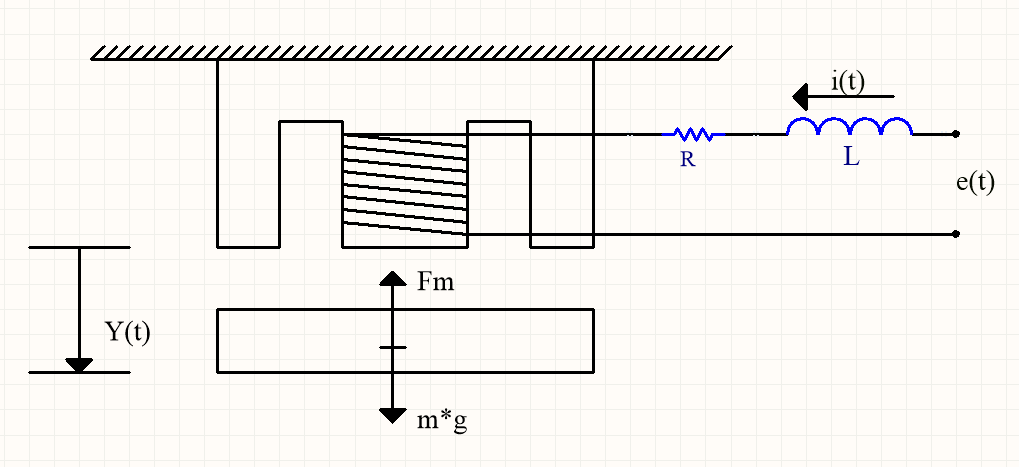
\includegraphics[width=\textwidth]{modelo-fisico.png}
	\caption{Modelado físico.}
	\label{fig:img_modelado-fisico}
\end{figure}

\noindent Se sabe que la fuerza correspondiente al peso del objeto es $F_{m}=m*g$. Por lo tanto, el electroimán debe generar una fuerza de igual módulo y sentido contrario para mantenerlo suspendido en estado de equilibrio. Esta fuerza se obtiene de la circulación de un flujo magnético entre el núcleo del electroimán y la pieza con forma de I. Para generar el flujo magnético se necesita una fuerza magnetomotriz.

%esto es otra cosa ya. hacer una intro de como se genera la fuerza magnética???
\noindent La fuerza magnetomotriz generada en el núcleo del electroimán es proporcional a la corriente que circula por su bobinado, y su módulo está dado por la ecuación \ref{eq_fuerza-magnetomotriz}. Para poder modelarla se debe realizar un análisis físico del actuador. 

\begin{equation} \label{eq_fuerza-magnetomotriz}
	F_{mm}=R_{m}*\phi=N*i	
\end{equation}

%mejorar este parrafo
\noindent En donde $R_{m}$ corresponde a la reluctancia del circuito magnético, $\phi$ indica la magnitud del flujo, es decir, la cantidad de campo magnético que atravies una superficie y $F_{mm}$ es la fuerza magnetomotriz (que es distinta a la fuerza magnética $F_{m}$). La ley de Hopkinson relaciona estos parámetros con la corriente que circula por el bobinado ($i$) y la cantidad de vueltas de su núcleo ($N$).


\noindent Por otro lado, la inductancia del bobinado está dada por la ecuación \ref{eq_inductancia_flujo}

\begin{equation} \label{eq_inductancia_flujo}
	L*i=N*\phi
\end{equation}


\noindent Como se ve en la figura \ref{fig:img_modelado-fisico}, el electroimán utilizado está compuesto por una pieza en forma de E y otra en forma de I, que se encuentran separadas por un espacio o gap de aire. Este circuito magnético se puede modelar como a un toroide con un corte o separación  de longitud $lA=2*y$, como se muestra en la figura \ref{fig:img_toroide}

\begin{figure}[H]
	\centering
	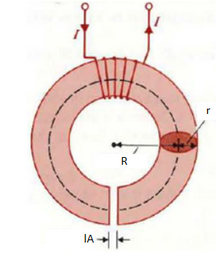
\includegraphics[scale=0.75]{toroide.png}
	\caption{Toroide con gap de aire.}
	\label{fig:img_toroide}
\end{figure}

\noindent Para el análisis se utiliza la ecuación \ref{eq_reluctancia} para modelar la reluctancia de un toroide sin gap de aire, con área transversal A, permeabilidad del material $\mu_{r}$ y longitud del circuito magnético $l_{h}$. 

\begin{equation}\label{eq_reluctancia}
	R_{m}=\frac{l_{h}}{\mu_{o}*\mu_{r}*A}
\end{equation}

\noindent Combinando las ecuaciones \ref{eq_fuerza-magnetomotriz}, \ref{eq_inductancia_flujo}, y \ref{eq_reluctancia}, se llega a la expresión de la inductancia del toroide:

\begin{equation}\label{eq_inductancia}
	L=\frac{N}{i}*\phi=\frac{N}{i}*\frac{N*i}{R_{m}}=\frac{N^	{2}*A*\mu_{o}*\mu_{r}}{l_{h}}
\end{equation}


\noindent Al agregar un gap de aire, se genera una discontinuidad en el medio magnético. Es decir, se genera una discontinuidad de distancia $l_{A}$ (longitud en el aire).

\noindent Según Maxwell, las líneas de flujo magnético son todas continuas. Es decir, no hay carga magnética como tal, a diferencia de los campos electrostáticos que sí los hay. Por lo tanto, el mismo flujo que circula por el material ferromagnético, es el que  está en el aire. 

\noindent Es posible que las líneas de flujo presentes en el gap de aire sufran de ensanchamiento provocando que las mismas no se mantengan constantes (efecto fringing). A efectos prácticos esto es despreciable ya que esta distancia es lo suficientemente pequeña dejando como sección transversal aproximada A.

\noindent Considerando que al haber un gap de aire, la reluctancia del sistema aumenta, por lo que se debe sumar, en serie a $R_{m}$, la reluctancia en el aire $R_{a}$. Por otro lado, $l_{h}$ prácticamente no se ve modificada ya que es una pequeña incisión en el flujo magnético. De esta forma, se obtiene la ecuación \ref{eq_inductancia_con_gap}.

\begin{equation}\label{eq_inductancia_con_gap}
L=\frac{N^{2}}{R_{m}*R_{a}}=\frac{N^{2}}{\frac{l_{h}}{A*\mu_{o}*\mu_{r}}+\frac{l_{a}}{A*\mu_{o}}}=\frac{N^{2}*A*\mu_{o}}{l_{a}+\frac{l_{h}}{\mu_{r}}}
\end{equation}

\noindent Sabiendo que $l_{a}$ es el gap de aire, se debe reemplazar por la distancia de separación entre las dos piezas magnéticas, la cual está representada por la variable y. En el caso de nuestro electroimán, las líneas de fuerza atraviesan dos veces y, por lo tanto $l_{a}=2*y$.

\noindent Además, considerando que en la ecuación \ref{eq_inductancia_con_gap} $\mu_{r}>>1$ entonces $2*y>>\frac{l_{h}}{\mu_{r}}$ y se obtiene la inductancia en función de la distancia del gap de aire y:

\begin{equation}\label{eq_inductancia_vs_y}
		L(y)=\frac{{N^{2}*A*\mu_{o}}}{2*y}
\end{equation}

\section{Cálculo de la fuerza magnética}

\noindent La fuerza magnética necesaria para mantener a un objeto en suspensión se puede encontrar a partir de la energía almacenada en un inductor y al considerar que esta es  igual al trabajo:

\begin{equation}\label{eq_energia}
	E(i,y)=W=\int{F_{m}*dy}=>F_{m}=\frac{\partial{E(i,y)}}{\partial{y}}
\end{equation}

\noindent Y sabiendo la expresión para obtener la energía que almacena un inductor en su campo magnético:

\begin{equation}\label{eq_energia_2}
	E(i,y)=\frac{L(i,y)*i^{2}}{2}
\end{equation}

\noindent Esto significa que la cantidad de energía que almacena el sistema es función del gap de aire. Combinando las ecuaciones \ref{eq_inductancia_vs_y}, \ref{eq_energia} y \ref{eq_energia_2}:

\begin{equation}\label{eq_fuerza_magnetica}
	\abs{F_{m}}=\frac{\partial{E(i,y)}}{\partial{y}}=\frac{i^{2}}{2}*\frac{\partial{\frac{{N^{2}*A*\mu_{o}}}{2*y}}}{\partial{y}}=\frac{i^{2}*N^{2}*\mu_{o}*A}{4*y^{2}}
\end{equation}

\noindent Como se puede apreciar en la ecuación \ref{eq_fuerza_magnetica} la fuerza es proporcional al cuadrado de la acción de control (es decir, de la corriente), e inversamente proporcional al cuadrado de la variable que se desea controlar (es decir, de la distancia). Por lo tanto, el problema adquiere un comportamiento sumamente alineal.

\section{Diseño del electroimán}

%¿sería conveniente hacer el diseño partiendo del electroimán que ya tenemos, y en base a eso determinar el peso que podemos levantar?
\noindent Se debe determinar qué dimensiones debe tener el electroimán a utilizar para que sea capaz de ejercer la fuerza magnética necesaria para mantener levitando el peso deseado.

\noindent Al analizar la ecuación \ref{eq_fuerza_magnetica} se puede observar que hay dos parámetros que son propios del electroimán: el área del núcleo A y la cantidad de vueltas del bobinado N. Para obtener una expresión de diseño, partimos de esta ecuación y la igualamos al fuerza ejercida por el peso que debe soportar ($\abs{F_{m}}=m*g$):

\begin{equation}\label{eq_fuerza_peso}
	m*g=\frac{i^{2}*N^{2}*\mu_{o}*A}{4*y^{2}}
\end{equation}

\noindent De la ecuación \ref{eq_fuerza_peso} podemos despejar el producto $N*i$ que es la fuerza magnetomotriz:

\begin{equation} \label{eq_n_por_i}
	N*i=y*\sqrt{\frac{4*m*g}{\mu_{o}*A}}
\end{equation}

\noindent Partiendo de la ecuación \ref{eq_inductancia_flujo}, reemplazando $\phi=B*A$ y considerando el caso de máxima inducción magnética ($i_{max}$):

\begin{equation}\label{eq_inductancia_densidad}
	L*i_{max}=N*B_{max}*A
\end{equation}

\noindent Luego, relacionando la ecuación \ref{eq_inductancia_vs_y} y \ref{eq_inductancia_densidad}:

\begin{equation} \label{eq_bmax}
	B_{max}=\mu_{o}*\frac{N*i_{max}}{2*y}
\end{equation}

\noindent Combinando la ecuación \ref{eq_bmax} y \ref{eq_n_por_i}:

\begin{equation}
	B_{max}=\sqrt{\frac{m*g*\mu_{o}}{A}}
\end{equation}

\noindent Finalmente:

\begin{equation} \label{eq_area}
	A>=\frac{m*g*\mu_{o}}{B_{max}^{2}}
\end{equation}

\noindent Con el objetivo de evitar la saturación del núcleo del electroimán en el caso que circule la máxima corriente, el área transversal debe cumplir con la expresión \ref{eq_area}. Para el cálculo se utiliza $B_{max}=0.7$ Tesla, que corresponde con la inducción máxima del acero de silicio. \colorbox{red}{CHEQUEAR}. Finalmente se obtiene:

\begin{equation}
	A>=20 cm^{2}
\end{equation}


\section{Diseño del electroimán}

\noindent El electroimán está construido por un núcleo de acero laminado con forma de E, que tiene un cable bobinado en su rama central, y otra pieza con forma de I.\colorbox{red}{poner imagen con dimensiones}. 
% 

Está construido por una laminación normalizada sin desperdicio 600. Estas son útiles ya que cada par de laminas E y I puede fabricarse a partir de una lámina de acero rectangular, de manera de que no se desperdicia material durante la fabricación. \colorbox{red}{poner figura}

 Está compuesto por dos piezas: una con forma de “E” y otra con forma de “I”. En su núcleo tiene un bobinado de 150 vueltas (N) de cobre esmaltado con un diámetro de $2.5$ mm. El núcleo es de sección cuadrada ya que esto maximiza el área mientras que disminuye el perímetro, reduciendo así la longitud media de las espiras y ahorrando material. 


\section{Diseño del bobinado}

\noindent Se desea dimensionar la cantidad de vueltas del bobinado y la corriente requerida para las condiciones del problema. Partiendo de la ecuación \ref{eq_n_por_i} y considerando un área transversal $A=25 cm^{2}$, y las condiciones de trabajo más exigentes ($y=5$ mm y $m=30$ kg):

\begin{equation}
	N*i_{max}=3060.69 
\end{equation}

\noindent Debido a que ya se dispone de un electroimán con $N=150$, según el resultado anterior, se impone una corriente máxima de $20.4$ A. Para poder tener cierto margen en la masa máxima soportada, se adopta una corriente máxima de $21$ A, lo que resulta en un $N*i_{max}=3150$.



\section{Expresión de inductancia linealizada}

\noindent Volviendo a la ecuación \ref{eq_inductancia_vs_y}, se realiza una expansión por serie de Taylor y se desprecian los términos de orden mayor o igual a 2, con el objetivo de llegar a una expresión lineal para la inductancia se obtiene:

\begin{equation} \label{eq_inductancia_lineal_teorica}
	L(y)[mH]=-2.2089*y[mm]+17.67 [mH]
\end{equation}

\section{Mediciones sobre el electroimán}

\colorbox{red}{esto iría acá??}

